\documentclass[12pt,letterpaper]{article}
\usepackage{mla}
\begin{document}
\begin{mla}{Paul}{English}{ENG 2010-002}{Professor Argyle}{\today}{Examining the GISTEMP Surface Temperature Study}

\section{Introduction}
In our lifetime and over the past few decades human consumption and energy use has exponentially grown along with the size of our populations. We're driving more cars, using mobile phones and computing devices, and producing more batteries than ever before. We power buildings throughout cities, and homes throughout suburbs in order to provide comfort. 

Typically most humans live for less than one hundred years, and barely make a blip on the global lifespan of our planet. It's easy to discredit our actions now and not realize the half-life involved in our energy consumption. Given the size of our population, it's easy for just one generation to make a large impact on our environment that will span generations after it.

In this paper we review some of the current data and research regarding environmental change, and we look at how consumer and industrial technology plays a part in the impact of our environment. 

\section{Methods}
There are several useful sources of information and data that relate to environmental change, and well-being. Currently we monitor surface temperature using satellites, and ground stations in order to record our recent history. In addition, we can drill for ice core samples in order to observe and infer on historical environmental data.

The NASA, Goddard Institute for Space Studies, performs a comprehensive report annually using surface temperature data gathered from satellites. This is called the GISS Surface Temperature Analysis, or GISTEMP. In the GISTEMP analysis, satellites collect surface temperature readings from stations around the globe, and the data is compiled and offered freely for anyone to learn from. This project began in the 1970s, in order to provide a report that measures global temperature change. By analyzing and collecting temperature data from global points we have been able to gain a greater understanding of the temperature change in our recent history.

Attempting to understand the global temperature patterns of a planet is not exactly a simple task, and there are many possible ways this data could be organized. The GISTEMP analysis does freely provide all the data used to compile their reports, yet it can be a little difficult to transform this information into a useful presentation format. However, the visual graphs and compiled statistics provided in their report are thorough and easy to understand. (``GISS")

\subsection{Visualized Temperature Anomaly}
The temperature data that we have in this analysis begins in 1880, and continues up to the current year of the published report. The core metric that is plotted along this time series is temperature anomaly, which describes the temperature change across the period of time observed. We are provided with Global Land Ocean Temperature plots, which provide an average temperature anomaly for each year, plotted as a function of time to allow us to see how observed temperature anomaly has changed over time (``GISS'' Fig. 1). For each year we also have an Annual Mean Surface Temperature Anomaly graph that allows us to see individual points of temperature data plotted by latitude and longitude across a global map (``GISS'' Fig. 2). This allows us to see temperature anomaly for any given year organized by the individual region or area of our planet.

\subsection{Other Data Alternatives}
In addition to modern temperature analysis, we can study drilled ice core samples, paleoclimatology, which hold clues into past global environments. Ice core samples contain contaminants that can be used to gauge global and regional levels of common greenhouse gasses. By calculating estimated CO2 levels found in ice samples and comparing these findings to other ice samples, we can observe what the environment was like before recorded temperature readings. Reports on ice core samples highly differ, and can be searched by individual researcher or global region. There is no comprehensive analysis that includes all the ice core data, that individual research organizations have collected. However, we can observe trends that are common from ice core sample to ice core sample in order to gain an empirical understanding. (``Heinberg'')

\section{Results}
The Global Land Ocean Temperature index is the most easily understood chart provided in the GISTEMP analysis (``GISS" Fig. 1). As mentioned before it provides averaged yearly  temperature anomaly plotted for each year starting at 1880. Inspection shows us a growing trend in this graph, indicating that temperature deviations are on average growing from year to year, with significant growth in the past few decades alone. This trend in anomaly provides evidence of increased temperatures, compared to years before.

\begin{center} % Figures
\begin{picture}(320,235)
\put(0,0){
\setlength{\fboxsep}{20pt}
\setlength{\fboxrule}{1pt}
\fbox{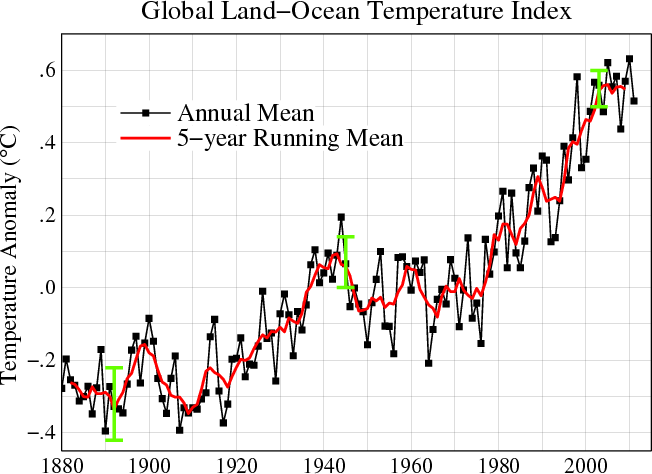
\includegraphics[scale=0.4]{global-land-ocean-temp-index-2011.png}}
}
\put(15,-15){Figure 1: Global Land-Ocean Temperature Index (``GISS").}
\end{picture}
\end{center}
\vspace{15 mm}

The Annual Mean Surface Temperature Anomaly which plots temperature anomaly by latitude and longitude across a map (``GISS" Fig. 2). By observing this graph we can see that global temperature anomaly is not the same across different regions of space, like the previous chart would have us believe. Using this viewpoint we are able to see a few new trends. Temperature anomalies above most of bodies of water have more stability than regions of land. Additionally, we're able to see that high temperature anomaly is most severe at both poles, with our northern hemispherical area over the Eurasian continent showing the highest points of temperature anomaly. This would suggest that these typically colder frozen areas are in fact warming up more than any other areas on the map.

\begin{center} % Figures
\begin{picture}(450,205)
\put(0,0){
\setlength{\fboxsep}{20pt}
\setlength{\fboxrule}{1pt}
\fbox{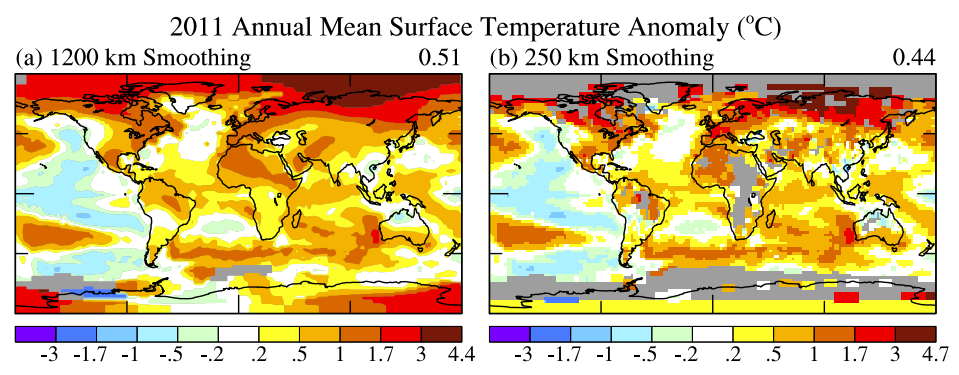
\includegraphics[scale=0.4]{annual-mean-surface-temperature-anomaly-2011.png}}
}
\put(15,-15){Figure 2: 2011 Annual Mean Surface Temperature Anomaly (``GISS").}
\end{picture}
\end{center}
\vspace{15 mm}

The data that we have from the GISTEMP analysis, though accurate, is far from perfect, and it's important to understand that though there are positive trends in global temperature warming, the data collection methods and analysis have changed and improved over the years. We can assume that the data collected in the past decade is more accurate and precise than that of past decades. The method of collecting and analyzing this data has also changed in a few ways, since it's inception in the 1970s. However, the report is accurate enough to allow us to use the trends shown as evidence for global warming, and we will likely continue to improve our methods of data acquisition and analysis over the coming years.

Adding support to the NASA surface temperature analysis, we can look additionally at historical data found in ice core samples. From an ice core sample we're able to measure Carbon Dioxide levels and gauge what impact it has on the current environment. We can also see that CO2, as well as other greenhouse gasses, have increased over the years (``Heinberg"). Richard Douthwaite explains that these changes both explain the growth in temperature, and they will also continue to influence the global surface temperatures. The increased temperature causes ice to melt, which releases gasses like methane. These gasses contribute to further greenhouse warming. The ice which also used to help reflect heat, is now ocean, which is darker and more prone to absorbing energy from the sun. This creates a snowball effect, multiplying the warming across the globe. Much of this warming has been linked to initial increased greenhouse gasses due to the combustion and consumption of fossil fuels (``Heinberg'' 54).

\section{Recommendations}

Understanding that our society can make large impacts in our global environment is one of the first steps of controlling and improving the world we live in. Only in our civilization's recent history have we been connected enough to gather these results and findings of our global environment. Paradoxically it is the technology that enables these findings that is also damaging and hurting our environment to begin with. Technological change and growth comes at a price as we use more natural resources in order to create these improvements. Our computers, our transportation, and our energy infrastructure all impacts the environment in finite measurable ways.

Luckily the solutions to these problems we are now discovering are numerous and can be accomplished by individual and organization both. Even now we are seeing greater understanding in global environmental issues in the general public, as well as initiatives to decrease wasteful consumption and conserve what we have for future generations. Companies that serve consumers with household goods can provide more efficient technologies. Walmart made a goal to sell 100 million CFL bulbs to consumers, which provides an estimated savings equivalent to removing 700,000 cars from the road (``WalMart''). Companies with a large fleet of fossil fuel burning vehicles can reduce their consumption in novel ways as well. UPS recently saved 3 million gallons of gas per year by optimizing the mapping algorithms they use to route packages (``UPS"). As individual consumers we can postpone buying that new mobile tablet, or high resolution laptop if we've already got something that fits the bill. The production of these devices, and the batteries used in them require large factories that pollute and negatively influence environmental change.

\section{Conclusion}
Data relating to recent environmental change shows that we are experiencing more increased temperatures than we have in recent history, and that these temperatures likely correlate to the increased amount of green house gasses in our environment. The production of these gasses are caused by many of our modern technologies. It is only through understanding these trends, and what the probable causes are, that will allow us to improve and positively impact our environment for generations that will come after us. We must focus every day on improving this awareness and decreasing our abuse of the environment we live in.

\begin{workscited}

\bibent
Goddard Institute for Space Studies. ``National Aeronautics and Space Administration." Data.GISS:GISS Surface Temperature Analysis (GISTEMP). NASA, 17 Feb. 2012. Web. 26 June 2012. $<$http://data.giss.nasa.gov/gistemp/$>$.

\bibent
Heinberg, Richard, and Daniel Lerch. \textit{The Post Carbon Reader: Managing the 21st Century's Sustainability Crises.} Healdsburg, CA: Watershed Media, 2010. Print.

\bibent
UPS. Public Relations. ``Right Turn at the Right Time." UPS Pressroom. UPS, 2007. Web. 21 June 2012. $<$http://pressroom.ups.com/About+UPS/UPS+Leadership/Speeches/\\D.+Scott+Davis/Right+Turn+at+the+Right+Time$>$.

\bibent
Wal-Mart. ``Wal-Mart Surpasses Goal To Sell 100 Million Compact Fluorescent Light Bulbs Three Months Early." Wal-Mart Corporate. Wal-Mart, 2 Oct. 2007. Web. 21 June 2012. $<$http://www.walmartstores.com/pressroom/news/6756.aspx$>$ .


\end{workscited}
\end{mla}
\end{document}
